\chapter{Obsah CD}
\label{pr:cd}
Adresárová štruktúra CD
\begin{itemize}
\item \textit{src} - Zdrojové súbory 
    \begin{itemize}
    \item \textit{app} - Zdrojové súbory aplikácie
    \item \textit{api} - Zdrojové súbory aplikačného rozhrania
    \item \textit{helper} - Zdrojové súbory aplikácie na ohraničovanie rán konzultantom
    \end{itemize}
\item \textit{demo} - Demonštračné súbory
    \begin{itemize}
    \item \textit{android} - Android aplikácia
    \item \textit{windows} - Windows aplikácia
    \item \textit{tutorial} - Video návod
    \end{itemize}
\item \textit{shots} - Snímky rán
    \begin{itemize}
    \item \textit{anotated} - Anotované snímky
    \item \textit{detected} - Výsledky detekcie
    \end{itemize}
\item \textit{text} - Text práce
    \begin{itemize}
    \item \textit{pdf} - Výsledný PDF dokument
    \item \textit{src} - Zdrojové súbory
    \end{itemize}
\end{itemize}

\chapter{Návod na inštaláciu}
Android a Windows aplikácia je dostupná na priloženom CD a Android aplikácia dokonca aj v obchode Google play. Aplikačné rozhranie beží na autorovom virtuálnom privátnom servery \url{http://194.182.70.49:5000/}. Avšak v prípade nutnosti, kedy by bolo požadované znovu nasadiť aplikačné rozhranie na server, alebo zostaviť aplikáciu je prítomný tento návod. 

\section{Nasadenie serverového aplikačného rozhrania}
Serverové aplikačné rozhranie vyžaduje pre svoj beh Python verziu 3.5.2 a MongoDB verziu 3.6.2. Pre nainštalovanie závislostí sa vyžaduje správca balíkov pip3 verzia 8.1.1. Po tom, ako cieľový stroj obsahuje všetky tieto programy, je možné spustiť skript instaler.sh, ktorý nainštaluje potrebné závislosti hlavne pomocou pip3 (skript je tvorený pre operačné systémy založené na Ubuntu, používa okrem pip3 aj apt-get). Následne je nutné spustiť MongoDB databázu pomocou príkazu \textit{mongod}, nastaviť cestu k hlavnému súboru (\textit{export FLASK\_APP=main.py}) a spustiť server pomocou príkazu \textit{flask run}. Server následne bude načúvať na porte 5000. 

\section{Zostavenie aplikácie}
Aplikácia pre zostavenie vyžaduje Node verziu 9.4.0 a správcu balíkov NPM verziu 5.6.0. Samotný Ionic je potrebné nainštalovať vo verzií 3.20.0. Po nainštalovaní rámca Ionic je potom možné spustiť inštalovanie závislostí pomocou príkazu \textit{npm install} v koreni adresára projektu a pridať Cordova platformy android a browser príkazmi \textit{ionic cordova platform add android} pre Android verziu a \textit{ionic cordova platform add browser} pre Windows desktop verziu. Pre zostavenie android aplikácie je nutné následne spustiť príkaz \textit{ionic cordova build android --prod --release}, alebo \textit{ionic cordova build browser --prod --release}. Desktopovú verziu je potom nutné ešte zabaliť do \textit{asar} archívu spustením skriptu \textit{electron/packager.sh}, ktorý vytvorí tento archív s aplikáciou pre Electron v zložke \textit{electron-dist} a následne tento archív priložiť k samotnému Electronu.

\chapter{Android aplikácia}
\label{pr:qr}
\begin{figure}[h]
      \centering
      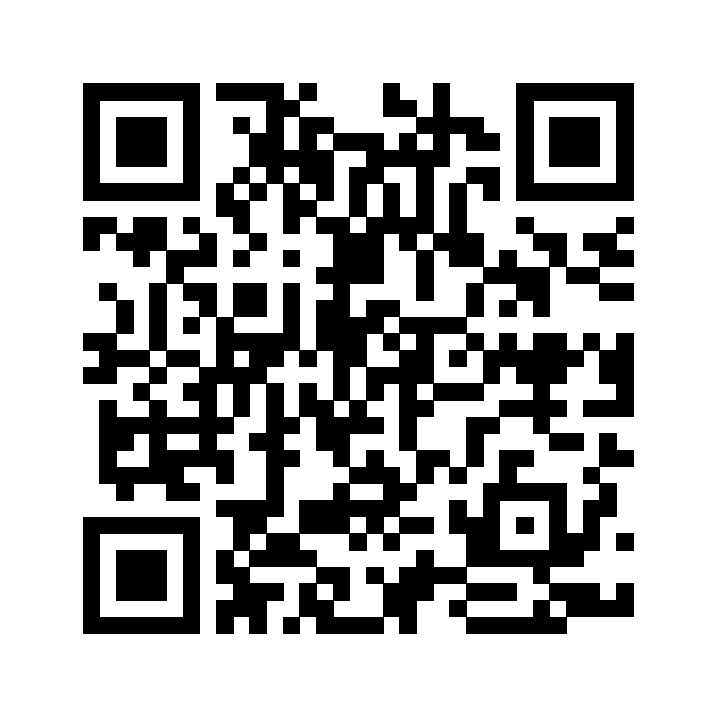
\includegraphics[scale=0.6]{fig/qr-play-google-com.eps}
      \caption{\href{https://play.google.com/store/apps/details?id=net.raiper34.wounddetector}{play.google.com/store/apps/details?id=net.raiper34.wounddetector}}
      \label{fig:qr}
\end{figure}
